For a thorough examination of the language, DEF has a language wiki,\cite{DEFWiki} however, a brief look is given below.  The DEF compiler is based on the Tapir branch of LLVM, that provides fork-join parallelism primitives.\cite{TAPIR,LLVM}  The front-end is principly written in OCaml, but includes some C++.

Likewise, the \texttt{defghi} utility is written in OCaml,\cite{DEF} and is described in the C Interface section.

Finally, the suite of microbenchmarks was developed in DEF and C with the driver in DEF.  The concurrent data structures selected for the suite were chosen for high performance and variety.

\subsection{Basic Syntax}

\begin{figure}[htbp!]
        \centering
        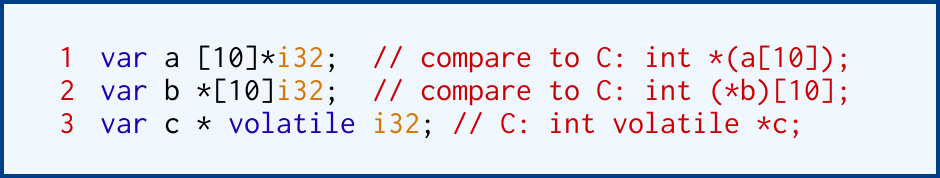
\includegraphics[scale=0.25]{gfx/types}
        \caption{Examples of variable declarations in DEF.  C allows the parentheses to be omitted in the first case, though they're provided to make precedence explicit.}
        \label{fig:types}
\end{figure}

Syntactically, DEF looks similar to C with the most apparent difference being that scopes are denoted by keywords instead of curly braces (e.g., \texttt{if} and \texttt{fi}, \texttt{do} and \texttt{od}, etc.) allowing curly braces to be repurposed for tuples.  Native types specify a bit width, so C's \texttt{int} on most systems corresponds to DEF's \texttt{i32}.  Types are also designed to read left-to-right, so the return type in a function declaration has been moved to the right using an arrow notation similar to ML-like languages or Go.  For more complicated types, fig.~\ref{fig:types} gives an example of left-to-rightness where no parentheses are needed to distinguish an array of pointers to integers (line 1) from a pointer to an array of 32-bit integers (line 2).

\begin{figure}[htbp!]
        \centering
        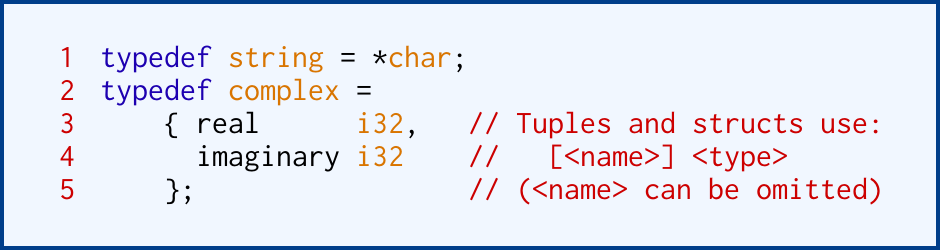
\includegraphics[scale=0.25]{gfx/typedef}
        \caption{Defining types with \texttt{typedef}.}
        \label{fig:typedef}
\end{figure}

Types are defined with the \texttt{typedef} keyword.  Figure \ref{fig:typedef} shows two examples: a C-style \texttt{string} type is defined on line 1, and a complex number struct is defined on lines 2-5.  The struct's actual definition is identical to tuple syntax, though tuples typically omit the member names.  Worthy of note is that tuples in DEF really are just anonymous structs, in keeping with the design goal of interchangeability with C.  Whereas in many languages tuples are allocated on the heap and garbage collected, in DEF they're allocated however a named struct would be in C.  Locating a struct or tuple on the heap requires explicit allocation.  Fig.~\ref{fig:window-find} provides a \texttt{window\_{}find} function declaration from the Harris lock-free linked list\cite{Harris} in Herlihy and Shavit,\cite{HSBook} as expressed in C (lines 2-6) and DEF (lines 9-10).  In both cases, the struct is returned by value on the stack.  A pointer, in both cases, would require explicit pointer syntax.

\begin{figure}[htbp!]
        \centering
        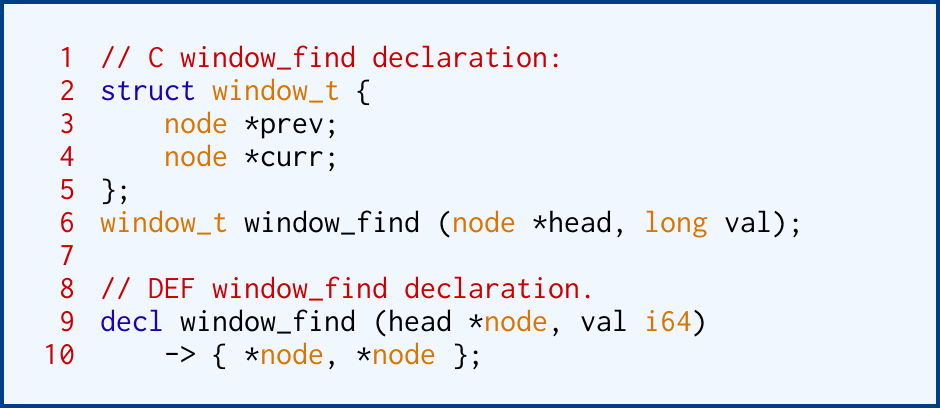
\includegraphics[scale=0.25]{gfx/window-find}
        \caption{Equivalent \texttt{window\_{}find} declarations in C and DEF.  The DEF tuple is an unnamed equivalent of C's \texttt{window\_{}t}.}
        \label{fig:window-find}
\end{figure}

Binary Read-Modify-Write (RMW) operations with sequential consistency can be expressed by applying an \texttt{atomic} modifier to the target operation.  Fig.~\ref{fig:atomic} shows an example of \texttt{atomic} being used to add into the variable \texttt{a}.

%% FIXME: Graphic should show new C atomics, not __sync_* functions.

\begin{figure}[htbp!]
        \centering
        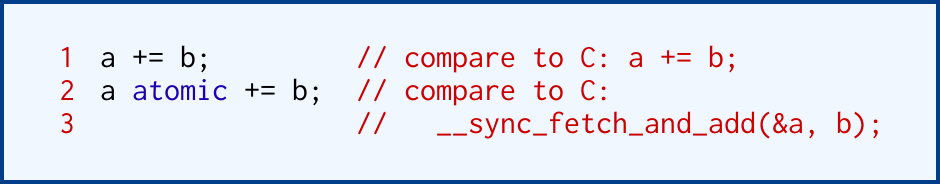
\includegraphics[scale=0.25]{gfx/atomic}
        \caption{Example of modifying a non-RMW operation to make it RMW in DEF.  The C version is GCC-specific.}
        \label{fig:atomic}
\end{figure}

\subsection{Allocation, Deallocation, and Reclamation}

DEF has no native allocator as distinct from C.  Allocating memory with \texttt{new} and deallocating it with \texttt{delete}, use \texttt{malloc} and \texttt{free}, respectively.  Since DEF's memory reclamation system is implemented using Forkscan, they implicitly use Forkscan's \texttt{malloc} and \texttt{free} wrappers, but the overhead of this indirection is undetectable in trials.  Independent of implementation, memory allocated with \texttt{new} is untracked.  Memory can be passed freely between DEF and C, and a pointer acquired in C through \texttt{malloc} can be deleted in DEF, and one acquired in DEF through \texttt{new} can be freed in C.

Moreover, \texttt{new} and \texttt{delete}, as applied to non-shared memory, are conveniences-only.  Mixing allocators or interfacing with a language with hooks to an external garbage collector is as trivial (or as complex) in DEF as it is in C because all memory is treated in exactly the same way.

The exception to this is in the use of \texttt{retire} to flag a pointer for tracking.  It's assumed that a retired node was allocated with the same allocator used by \texttt{new}.  Implementation-wise, Forkscan requires knowledge of the \texttt{free} and \texttt{malloc\_{}usable\_{}size} corresponding to the \texttt{malloc} that was used to acquire the memory.  More broadly, it's hard to see how any implementation could call the correct \texttt{free} on a retired node unless it corresponded to the known \texttt{malloc}, and this isn't especially burdensome to programmers.

A final restriction on \texttt{retire} is that it may only be called on a pointer, once.  If multiple threads retire the same memory, the behavior is undefined.  In practice, it acts like a double-free because the reclamation system may perform a double-free.  A good usage model is the thread that successfully removes a node from the concurrent data structure is the one that should retire it.  This makes its use intuitive because code looks like the familiar serial model where \texttt{retire} is replaced by \texttt{delete}.

Forkscan was modified to accommodate these semantics.  When Forkscan completes a memory sweep, it creates a pool of pointers known to have no outstanding references in the user program.  As designed, every call to \texttt{forkscan\_{}malloc} first frees a few of these pointers.  But this creates a dependency on \texttt{forkscan\_{}malloc}.  If a C module naively, repeatedly calls \texttt{malloc}, even from the correct allocator, and gives the memory to a DEF module that retires it, unless the DEF module is also independently allocating its own memory with \texttt{new}, none of the retired memory will ever be reused.  This is a practical leak.  The modification moved the burden from \texttt{forkscan\_{}malloc} to \texttt{forkscan\_retire}, eliminating the dependency.

This produced no discernable difference in performance.  The reasoning for the original design was that freeing memory and then immediately allocating would likely return a pointer to memory that was already in the cache.  High performance allocators tend to have this property.  Changing the location of the burden didn't affect performance because, even if \texttt{malloc} wasn't called immediately after \texttt{free}, the delay between retiring and allocating memory wasn't very great, and the allocated memory was probably still in the cache.  Since some of the concurrent data structures tested were among the most high-performance known, we reason that the change has little or no effect on performance.

\subsection{C Interface}

C++ is the gold-standard for interfacing with C.  As mentioned above, C header files can be included directly into C++ files, and C++ functions can be declared with C linkage.  Features like templates, classes, and member functions of structs, can't be exported to C, but anything C-like can be.  Given DEF's syntactic differences, even for features it holds in common with C, sharing DEF interface (\texttt{.defi}) files directly with C is impractical.  However, most of the function-level features have a one-to-one correspondence with C.  Therefore, the compiler is accompanied by a utility, \texttt{defghi}, for generating headers and interface files from DEF source files.

Generating headers and interface files is assisted by a formal approach to module interfaces.  A subtle distinction from C is that DEF types, functions, and globally-scoped variables are local to the module in which they appear, by default.  C's default is external visibility, and local symbols must be marked \texttt{static} by the programmer.  In contrast, DEF requires programmers to mark symbols with \texttt{export} in order to make them visible.

Since the differences are syntactic, generating header files from \texttt{defghi} is simple.  Any type, global variable, or function marked \texttt{export} has its declation unparsed into C and pretty-printed into the header.

The other direction, importing C definitions into DEF, involves recognizing headers by filename extension and passing them through a C parser.  Clang, the LLVM C compiler, collects all type definitions and function and global variable declarations, and DEF converts them into its own internal representation.  Therefore, DEF can import C headers directly as if they were native DEF.

There are two limitations to this: DEF can't import actual C functions (as opposed to function declarations), and C macros aren't resolved except where they appear in a header file itself.  In the first case, functions in header files are a planned feature that was deprioritized since they're uncommon in the C standard library, and it was reasoned that high performance programmers often do intermodule optimization, negating the value of putting them in headers.  In the second case, DEF does not yet have macros of its own, and a naive implementation of incorporating C macros might conflict with a well-designed DEF macro language.  Since C macros are simple text-substitution, integration into a language with a different syntax is another problem, altogether.

Even with the current limitations, however, DEF is able to import the C standard libraries, use their types, call their functions, and access their global variables.

\subsection{Concurrent Data Structures}

The structures selected are all sets, and the main benchmark driver randomly adds and removes nodes from them at a specified update rate.  It also includes two priority queues with their own driver.

\paragraph{Skip List} A fixed-height lock-free skip list was included as a well-known probabilistic concurrent data structure.  Each node contains one value, and the nodes are arranged in a list with a set of one or more forward pointers.  Each forward pointer points to the next node with at least that height, and the height averages two.  Operations take logarithmic time, as they would in a binary tree, but tend to have better cache usage.  A node is retired by the thread that swings the lowest height pointer during removal; a one-line change to the algorithm as described in Herlihy-Shavit.\cite{HSBook}

\paragraph{Hash Table} The lock-free separate chaining hash table performed favorably in Michael's tests.\cite{HashTables} Each bucket in the hash table contains a lock-free linked list based on the (Harris/Fraser list). The list at each bucket is sorted and allows for early search termination. Like the Harris list a window of nodes is kept for insertion and removal. Nodes in the list are removed by marking the current node's next pointer, effectively locking that node, then swinging the previous node's next pointer to the next pointer of the current node being removed. This stops another node inserted in front of the current node being deleted. Other threads which see a marked next pointer help remove the makred node from the list, making the remove operations cooperative and lock-free.

\paragraph{Binary Tree} The fast concurrent lock-free binary search tree by Natarajan and Mittal is a recent concurrent data structure that operates by marking edges rather than nodes.\cite{LFBinaryTree} The algorithm is relative simple and fast due to the lack of an active rebalancing algorithm. Rebalancing algorithms are a source of contention as some require a potentially global data-structure reorganisation. The data-structure is also an external binary tree, meaning the values of the set are stored in the leaf nodes rather than throghout the tree. The internal nodes are only for routing and serve no other purpose. The work-horse of the data-structure is the \texttt{seek} method. Like the Harris linked list, \texttt{seek} constructs a window of the tree while searching. \texttt{Seek} will exclude nodes that have been marked for deletion as those nodes cannot be valid ancestors when removing. The tree contains nodes which are never removed so that there will always be a valid node family tree. Removing a node is a two stage process, first the node has its parent's edge to it marked and then marking the egde of the node's sibling and successor. Once both edges (of the parent) have been marked no other modifying operations can occur and the parent (an internal routing node) and the node to be removed can be removed. (talk about retiring)

\paragraph{Shavit Lotan Queue} This was included as an example of a skip list-based priority queue.\cite{ShavitLotanQueue} The Shavit Lotan Queue is a lock-free priority queue data-structure where the \texttt{pop-min} method traverses the lowest level of the skip list. Since the skip list is a series of sorted linked lists, with the lowest level containing all values, threads can remove the top items from the list which have the highest priority. Deletion is done via logically, using the atomic swap (other similar CAS) to mark a node as deleted and then physically removing that node then or sometime after. Timestamps can be added to each node in order to make the list linearisable (cite), otherwise the structure is quiescently consistent (cite).

\paragraph{SprayList} Finally, the SprayList priority queue was implemented.\cite{SprayList}  Like the other, this is based on a skip list, but the node to remove is selected probabilistically from near the beginning to reduce contention. This probabilistic walk is refered to as the \textit{spray} and is paramount to reducing contention from threads. The SprayList is a relaxed concurrent data-structure whereby \texttt{pop-min} will remove from a range of top items in the list. The range and other parameters of the spray are initialised by the number of expected threads (concurrency) acting on the list. Because nodes closer to the beginning are less likely to be \textit{landed-on} after the spray padding nodes are added to the beginning of the list. Once the SprayList sprays it will continue in the same fashion as the Shavit Lotan Queue and traverse the lowest level of the list until a non-deleted node is found. Under high contention the SprayList can scale significantly better than other concurrent priority queues. As in the skip list, the node is retired by the thread that swings its lowest height pointer. 
